%!TEX root = thesis.tex 

\chapter{Towards a Better Web} \label{cha:Towards a Better Web}
	\paragraph{}
	In 1945, Vannevar Bush wrote "As We May Think"~\cite{Bush1945As}, an essay describing the concept of the Memex. He hoped to convert information, which was generated at an increasingly fast rate, into knowledge. His concept of the Memex envisioned a device that would allow people to store all their books, records, or any other form of data. The device would help the users to consult their database with increased efficiency and speed. Besides the stored data the users could store self created associative links, and this would be the reason for the increased speed and efficiency. These associative links would point from one data source to another, which in essence was an early form of hypertext. However, different to current implementations of hypertext technology, the associative links could be stored separated from the data source. The idea was that it would be easy for two users to share their database, as well as their self-created links between the data. This would help people working in the same domain to share their findings through these externally saved links.
	\paragraph{}
	Current hypertext technology attempts to reproduce this concept of creating associative links between content resources. The major difference however is that in the original concept of the Memex these links could exists next to the data source. This means that even if you could not alter the content of the document to, for example, add a link to another document, you could still copy the document to your own device. You could then save a link between this document and any other document you had in your device externally on a microfilm. This is an elegant concept that was lost when hypertext and HTML standards came to exist. In the current standards the distinction between content and metadata is missing and hyperlinks are an integral part of the document itself. A third party consumer of the content could not add links to the document which would hinder the user in maintaining a associative overview of the available information. Instead the author dictates what documents are associatively linked to the content he created.
	\paragraph{}
In the HTML standard, for example, one has to put embedded anchor tags with a \code{href} attribute in the page source in order to link two documents together. The readers cannot easily add more links when coming across another relevant document. If they wanted to do this, they would have to contact the original authors of the page and ask them to add this extra link to the page, which is bothersome and in most situations not a viable option.
\section{Alternative Tools} \label{sec:Existing Tools}
	\paragraph{}
	A couple of research groups~\cite{van2001open}\cite{phelps2000robust}\cite{pant2003deriving} have already identified similar problems with the current HTML linking mechanism introduces and many tools~\cite{bottoni2004madcow}\cite{annotea}\cite{naing2002ontology} have already been developed to mitigate some of these problems. These tools allow users to annotate existing web pages with text, add custom links to web pages on which they have no authoring rights or add more semantic information to hyperlinks. Of course these annotations and custom links are stored locally so they are not visible for other users.
	\subsection{Annotea} \label{sub:Annotea}
		\paragraph{}
		Annotea\footnote{\url{http://www.w3.org/2001/Annotea/}} is an RDF~\cite{klyne2004resource} standard created by the W3C LEAD (Live Early Adoption and Demonstration) project under the Semantic Web Advanced Development (SWAD). Annotea enhances collaboration via shared metadata-based web annotations, bookmarks and the various combinations thereof. These annotations can be comments, notes, explanations, or other types of external remarks that can be attached to any web document or a selected part of the document without actually changing the document. When the user requests the document they can also load the annotations attached to it from a selected annotation server or several servers and see what his peer group thinks. Similarly, shared bookmarks can be attached to web documents to arrange them under different topics for future reference, to help find related material and to collaboratively filter bookmarked material.\cite{annotea}\cite{koivunen2003annotea}\cite{koivunen2005annotea}
		\begin{figure}[h]
		\centering
		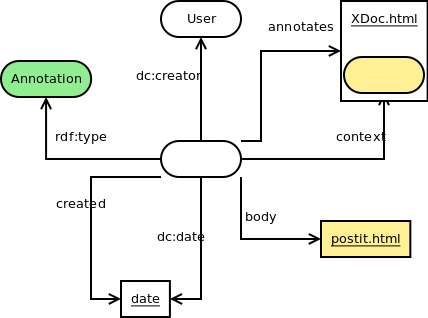
\includegraphics[width=\textwidth*4/5]{stateoftheart/rdfAnnotea.png}
		\caption{RDF model of Annotea's annotations}
		\label{overflow}
		\end{figure}
		\paragraph{}
		Annotea is open; it uses and helps to advance W3C standards when possible. For instance, we use an RDF-based annotation scheme for describing annotations as metadata and XPointer~\cite{DeRose2001} for locating the annotations in the annotated document. Similarly a bookmark scheme describes the bookmark and topic metadata.
		\paragraph{}
		Annotea is part of the Semantic Web efforts. Providing an RDF metadata-based extendible framework for rich communication about web pages while offering a simple annotation and bookmark interface. The annotation metadata can be stored locally or in one or more annotation servers and presented to the user by a client capable of understanding this metadata and capable of interacting with an annotation server over the HTTP service protocol.

	\subsection{Amaya Browser} \label{sub:Amaya Browser}
		\paragraph{}
		The first client implementation of Annotea is W3C's Amaya, a combination of a web editor and browser\footnote{\url{http://www.w3.org/Amaya/}}. Amaya is a tool used to create and update documents directly on the Web. Browsing features are seamlessly integrated with the editing and remote access features in a uniform environment. This follows the original vision of the Web as a space for collaboration and not just a one-way publishing medium.
		\paragraph{}
		Work on Amaya started at the W3C in 1996 to showcase web technologies in a fully-featured web client. The main motivation for developing Amaya was to provide a framework that is able to integrate as many W3C technologies as possible. It is used to demonstrate these technologies in action while taking advantage of their combination in a single, consistent environment.
		\paragraph{}
		Amaya started as an HTML + CSS stylesheets editor. Since that time it was extended to support XML and an increasing number of XML applications such as the XHTML family, MathML~\cite{carlisle2010}, and SVG. It allows all those vocabularies to be edited simultaneously in compound documents.
		\paragraph{}
		Amaya also includes a collaborative annotation application based on the Resource Description Framework (RDF), XLink, and XPointer as described by the Annotea standard. The Amaya browser was mainly used to showcase new features of the W3C standards and as a result the tool is specialised for the creation of hyperlinks.
		\begin{figure}[h]
			\centering
			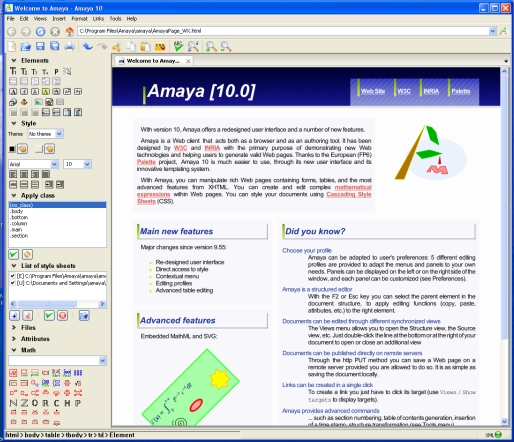
\includegraphics[width=\textwidth*4/5]{stateoftheart/amaya.jpg}
			\caption{The amaya browser}
		\end{figure}
	\subsection{Madcow} \label{sub:MadCow}
	\paragraph{}
	Madcow~\cite{bottoni2004madcow} is an acronym for \squote{Multimedia Annotation of Digital Content Over the Web} and was developed at the University of Rome: La Sapienza as a plugin for existing web browsers. The plugin uses a client-server architecture that allows users to save their created metadata to a remote server from where it can be shared with other users. The goal of the tool was to create an easy way for members of communities to share their findings and interests with each other.
	\paragraph{}
	The functionality of Madcow consist of reading, creating, saving, updating and retrieving multimedia annotations but does not allow the creation of hyperlinks between content.
	\begin{figure}[h]
		\centering
		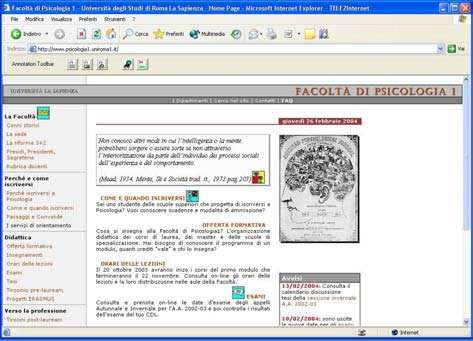
\includegraphics[width=\textwidth*4/5]{stateoftheart/madcowBrowser.png}
		\caption{The MADCOW plugin}
	\end{figure}
	\begin{figure}[h]
		\centering
		\begin{subfigure}[b]{\textwidth*2/5}
			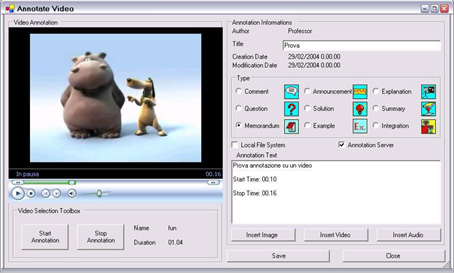
\includegraphics[width=\textwidth]{stateoftheart/madcowAnnotation1.png}
			\caption{Video annotation}
		\end{subfigure}
		\begin{subfigure}[b]{\textwidth*2/5}
			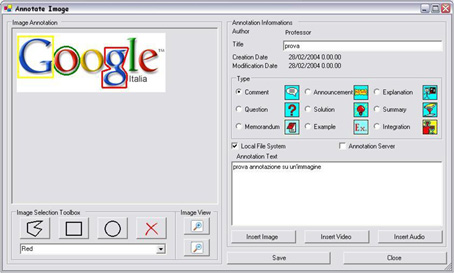
\includegraphics[width=\textwidth]{stateoftheart/madcowAnnotation2.png}
			\caption{Image annotation}
		\end{subfigure}
		\caption{Annotations in MADCOW}
	\end{figure}
	\subsection{iWeb} \label{sub:iWeb}
		\paragraph{}
		iWeb is a front end for iServer~\cite{norrie2005information}\cite{signer2008fundamental}, a collaborative metadata server that stores linking metadata for different resources. iWeb is implemented as an add-on for Firefox, enabling the user to highlight a part of the web page and create an annotation or a link to another web page. This metadata is then stored in iServer's back end. The main problem with iWeb was the fact that it was implemented as a plugin, and was therefore highly reliant on the inner workings of Firefox at that time. Web browsers tend to change their inner workings rather quickly to accommodate for changes in the web standards or to increase performance. As a result, iWeb was strongly bound to a specific version of Firefox and would not work in the future without continuous updates. Instead, we opted to start over, and make the tool as generic and independent as possible. In a way, iWeb was the predecessor of our current tool, in that it gave us a lot of valuable insights in how we could visualise the metadata on the Web.
\section{Newly Introduced Issues} \label{sec:Newly Introduced Issues}
	\paragraph{}
	One characteristic all the tools we introduced share is the fact that they were intended for a single user. At best the data is stored on a personal server, so that peers can connect to it and share their findings and even in these cases the amount of people using a single database would be fairly limited. As a result of this design decision the users can manually manage the metadata that is created. If a page becomes to cluttered the users could simply remove a couple of unneeded links, or regroup some similar ones.
	\paragraph{}
	When dealing with a truly collaborative system, where users of all backgrounds share their metadata on one large central server, this management cannot be done manual any more. These issues where previously masked because of the setting in which the tools were supposed to be used. Drastically changing the intended setting would inevitably lead to new issues that need to be addressed.
	\subsection{Visibility} \label{sub:Visibility}
	\paragraph{}
	The first major issue a multi-user system needs to deal with is the visibility of a web page. Imagine the front page of a popular newsletter website that has thousands of hits per day. A good portion of these users will have additional information to share with the community, and they will do so by creating a link to a different article. But as we can imagine, the community will soon generate such a large amount of metadata that visualising all of this data on the web page will become unreadable. When another user then views the page, it will be difficult for them to see the actual content through the seas of extra data, so the usability and readability is reduced because of the tool.
	\paragraph{}
	Most tools will visualise the origin and destination of the links within the content of the page by some form of highlighting or underlining the relevant parts of the text and since there is so much data to be visualised, it is possible that the entire document will be highlighted. A completely highlighted page is just as useful as a plain one.
	\paragraph{}
	New users will therefore arrive on a page that is completely cluttered with metadata that adds nothing to the user's experience and will actually hamper the user in the reading of the original text.
	\paragraph{}
	This means that once the amount of visitors is high enough, there is a potential danger that the system will work against itself. At that point the user would be better off not using the tool at all. Therefore a better way needs to be found for visualising the potential vast amount of metadata without overwhelming the user with too much data.
	\paragraph{}
	A second problem with trying to visualise the source and destination of the hyperlinks occurs when we have hyperlinks with overlapping sources. Two hyperlinks may be created where the source selection of the first link overlaps with the source selection of the second one. Naively visualising these two links will result in a highlighted area of text with no distinction as to where the first selection ended, or the other selection began. The same effect happens when two selections are exactly next to each other, and when one of the selections is completely within a second one. Visualising these types of scenarios directly on the page can be a challenge and may require even more metadata, such as layering, to be rendered in a readable way.
	\begin{figure}[h]
		\centering
		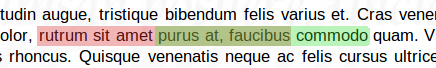
\includegraphics[width=\textwidth*4/5]{stateoftheart/Overlapping.png}
		\caption{Two overlapping selections}
		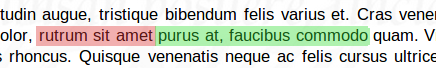
\includegraphics[width=\textwidth*4/5]{stateoftheart/Connecting.png}
		\caption{Two connecting selections}
		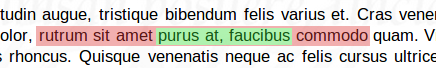
\includegraphics[width=\textwidth*4/5]{stateoftheart/Encapsulating.png}
		\caption{A selection surrounding another}
	\end{figure}
	\subsection{Scalability} \label{sub:Scalability}
		\paragraph{}
		A second major issue that was masked because the tools were intended to be used by a single user or a small group of users, is the issue of scalability. When more users are using the same shared database, the amount of metadata that the tool needs to handle increases. Searching for specific annotations or hyperlinks will become increasingly difficult. This is not only a visualisation problem but a technical problem as well. For example, the Amaya browser allows users to share a sort of bookmarks on pages, which can function as hyperlinks that are not rendered on the page. The user can then search through the bookmarks on a certain page, but when the amount of bookmarks becomes to high, more intelligent ways of searching need to be introduced to mitigate this problem.
		\paragraph{}
		The authoring of new links will become another problem that is strongly linked to the searching problem. The community would not want users to create hyperlinks that are already in the system. But if it is difficult to search whether a specific hyperlink already exists, it is difficult to detect whether the newly authored link is a duplicate or not. Therefore the tool needs to take into account that the creation of duplicates is a possibility and act accordingly.
		\paragraph{}
		This problem did not occur when the tool was only used in the simpler single user setting, because the amount of data that needs to be managed is significantly smaller than when the tools is being used by hundreds of users simultaneously.
	\subsection{Lack of Overview} \label{ssub:Lack of Overview}
		\paragraph{}
		Even in small groups of users where the metadata might not clutter the entire page, it can still cause trouble for users looking for extra information regarding a subject on the source page. For example, the users are not interested in blog posts or videos on this particular topic, instead they would like to find scientific papers that provide more information. With all the links and metadata rendered on top of the page, it is difficult for the users to find the type of links they are interested in. It might be possible that the sentences the users are interested in are highlighted, but the links point to a YouTube clip instead of the PDF file they are looking for. This problem stems again from the fact that all this metadata is simply rendered in one place and there is no real way of filtering the types of links that the users are interested in.
		\paragraph{}
		The fact that the types of links cannot be filtered, together with the fact that all the different links are rendered in the same way, results in a lack of overview of what the page actually offers in terms of extra information. But the issue does not end there: users can only look at the structure of the page, and links are rendered within this structure. Because of this limitation there is a lot of interesting information that is not easily accessible. If we want to know what different websites a particular website links to, in other words: what are the websites that are strongly correlated with the current website, it is not an easy task to find out.
		\paragraph{}
		Therefore the larger structure of the metadata is lost as we are giving preference to the structure of the page instead. As a result it is difficult to look at the big picture of the metadata, and an overview of the metadata is lacking.
	\subsection{Suboptimal Use of Data Dimensions} \label{ssub:Suboptimal Use of Data Dimensions}
		\paragraph{}
		All this metadata has a multitude of dimensions by design. For example, the domain or web page it links to, the amount of users that followed the link, the amount of links that go to the same domain from this source document, how long ago this link has been created, and much more. However, by rendering it directly on the page, most of these dimensions are not used at all. The main dimension used in this visualisation is the location of the origin of the hyperlink. When we look at a link, we know exactly where the author of this link has intended it to appear and we know that this particular piece of content provides a context for the linked document. Other than this information there is little of the extra dimensions that is used in this visualisation. Imagine the same scenario as before, where the users are only interested in scientific papers in the PDF format. One thing these tools could do is only render the metadata for links that point to PDF files or present all different types of links in a different colour. Both options have their benefits and drawbacks. In the first scenario we may find only the intended PDF links, as we requested, but this would make it so that a lot of data that is available for the user is just not shown. One particularly interesting part of the document that the user wants to read more about has no links on it. So the users might have to look for this extra information by themselves bypassing the complete goal of the tool in the first place. However it might be the case that there are some links to blog posts in this section. Even though the user prefers scientific papers, they might still be interested in other media if the first option is not available. The second option is to show all metadata on the page but use this extra data type dimension to colour code the links on the page. This results in too much data being rendered and on top of that it is rendered in all kinds of different colours, again overwhelming the users.
		\paragraph{}
		The main problem is that the visualisation uses the spatial dimension as the most important one. They render the data based on the location of the origin of the links first, and after this dimension is rendered can try to add different dimensions, such as file type. There is no way for this type of visualisation to change the priority of the used dimensions. If the user is far more interested in the type of data, and after that the location of the link in the current document, there is no way to do this.
		\paragraph{}
		Even worse is the fact that some dimensions of the metadata simply cannot be used in this way. To determine how tightly two web pages are linked together based on the amount of links between them, we can analyse the metadata using an external tool but we cannot show this information directly to the user when they are browsing the web page using these tools. This information if often requested and is available in the metadata, it just cannot be used properly because the tool gives preference to the spatial dimension before anything else.
	\subsection{Copyright} \label{sub:Copyright}
		Another feature some of the tools implement is the possibility to transclude content of hyperlinks when rendering a web page. Instead of rendering a link pointing to a paragraph, the paragraph will be rendered where the link was defined. This is a nifty feature, and it will give a more complete picture of what extra information is available through the hyperlinks.
		\paragraph{}
		Aside from the visualisation issues, a non-technical issue arises with this feature. If the tool allows transclusion of content that is not necessarily provided by someone who owns the copyright on the content and the tool then transcluded this content on another web page, it is violating the copyrights of the transcluded content.
		\paragraph{}
		Is the user not allowed to create the hyperlink between these two web pages, or is the tool not allowed to transclude the content for this particular web page? Should the tool ask the author of the web page whether he is allowed to transclude its content or not? Should there be no transclusion at all to bypass this problem from the start? These are only a handful of the issues that can arise in tools where sharing and transclusion is a core feature.
		\paragraph{}
		There is no fixed answer to these questions but this should definitely be taken into account in the design of such tools. The tool can, for instance, allow websites to specify if they would like to be transcluded or not. If no information is available for a particular website, the tool will fall back on a default of rendering a hyperlink and leave the transclusion out. The tool could also transclude the content, but make sure that the original source is mentioned in the transcluded content. These examples show that there it not a fixed solution to handle these issues. But a well defined tool can certainly help to avoid serious copyright and ownership issues.
	\subsection{Side Effects} \label{sub:Side Effects}
		\paragraph{}
		The tools work well when used on a small scale, which is their intended setting, but the benefits quickly dwindle when too many users are creating metadata in the same shared database. For a small group of users that have the same interests or look for more information in the same sources, these tools can work great. But when too many users with diverse interests are dumping data in the same database, it will most likely hinder the users more than help them. As a result, these tools are best used on a smaller scale and within closed environments.
		\paragraph{}
		If we attempt to use the tools in a real multi-user setting, all the above mentioned problems will occur sooner or later. Pages will get cluttered with metadata, resulting in unreadable websites. Looking for new information on a specific topic will be cumbersome because there is simply so much data, and no real way of filtering or searching through it. In the end people might use the tools by turning everything off until they really cannot find something they are looking for. They will then turn the system back on and go through the painstaking process of browsing through the vast amount of data to see if the information they are looking for is in the system.
		\paragraph{}
		This defeats the purpose of the tools completely and will create a cascade of negative effects on the usability of the tool. If many users find that the tool hinders their search for additional information, they will stop using the tool as intended. As a result they will most likely stop authoring additional information, which will lead to a disengagement of a big part of the community. This will result in creation of less hyperlinks. Some people will then not find the additional information they are looking for and maybe stop using the system as well. This is a self-reinforcing cycle and eventually the tool will offer no real help to most users.
		\paragraph{}
		These problems have not been addressed by existing tools simply because the tools were intended to be used by a single user. This was of course in most cases a design choice, but it masked some important issues nonetheless. We can however analyse these design choices and by doing so we identified some key issues that stem from these design choices. Taking what we have learned from other tools, we can use this information to create a tool that will address these problems and this will eventually result in a better user experience and a tool that will promote collaborative annotating and hyperlinking of web pages.

	\section{Summary} \label{sec:Summary}
	\begin{center}
		\begin{tabular}{|p{3.5cm}||c|c|c|c|c|}
			\hline 
			\rowcolor{lightgray}Technical													& HTML5 & Annotea & Amaya  & Madcow & iWeb   \\ \hline
			\hline                                                                                                \hline
			\cellcolor{lightgray}Separated Metadata File					&        & \cmark & \cmark & \cmark & \cmark \\ \hline
			\cellcolor{lightgray}Collaboration										&        & \cmark & \cmark &        &        \\ \hline
			\cellcolor{lightgray}Centralized Server								&        & \cmark & \cmark &        & \cmark \\ \hline
			\cellcolor{lightgray}Extensible												& \cmark &        &        &        &        \\ \hline
			\cellcolor{lightgray}Search Function									&        &        & \cmark &        &        \\ \hline
			\cellcolor{lightgray}Spatial Dimension Preference			& \cmark & \cmark & \cmark & \cmark & \cmark \\ \hline
			\hline                                                                                                \hline
			\rowcolor{lightgray}Visual														& HTML5 & Annotea & Amaya  & Madcow & iWeb   \\ \hline
			\hline                                                                                                \hline
			\cellcolor{lightgray}Inline Rendering									& \cmark & \cmark & \cmark & \cmark & \cmark \\ \hline
			\cellcolor{lightgray}Overlapping Selections						&        & \cmark & \cmark &        & \cmark \\ \hline
			\cellcolor{lightgray}Transclusion											& \cmark &        & \cmark &        &        \\ \hline
			\cellcolor{lightgray}Structural Overview of Metadata	&        &        &        &        &        \\ \hline
			\hline 
		\end{tabular}
	\end{center}
	\paragraph{}
	As illustrated above, all of these tools address some of the issues with the limitations discussed in Chapter \ref{cha:Limitations of Linking Techniques}. The main focus of almost all the tools is the separation of the linking metadata from the content of the document. This is not surprising and represents a major step in the right direction. The tools may also address a couple of other issues but there is no all round best solution and we will need to weigh the pros and cons to choose the appropriate tool.
	\paragraph{}
	Another interesting trait all the tools have in common, is the fact that they all render their metadata inline. This is no improvement over standard HTML and this contributes to many limitations these tools still have such as the lack of structural overview of the metadata.

